\section{Anhang}

%Diese Latexvorlage ist auf Basis der Vorlage des \gls{IUMS} Instituts der technischen Hochschule Karlsruhe entstanden und wird nun als eigene Version der Steinbeis Universität weiterentwickelt.

Der Anhang enthält Inhalte, die den Lesefluss im Text beeinflussen würden, beispielsweise sperrige Tabellen oder größere Quellcodebeispiele. In diesem Falle wird er für einige Hinweise genutzt. Eine Arbeit kann auch mehrere Anhänge enthalten, sie sind dabei gleichrangig mit Kapiteln, welche selbst wieder Abschnitte enthalten können.

\subsection{Schriftliche Ausarbeitung}
Beim Anfertigen einer wissenschaftlichen Arbeit mit \LaTeX{} wird viel Arbeit zur regelgerechten und konsistenten Einhaltung der Form bereits durch das Satzsystem geleistet. Darüber hinaus sind einige Hinweise zu beachten:
\begin{itemize}
	\item Die Angabe von Referenzen auf das Literaturverzeichnis erfolgt mit \texttt{\textbackslash{}cite\{\}}, wobei die Quellen einzeln \cite{knuth.literate84} oder gruppiert \cite{knuth.literate84,nm.epinjava,lamportlatex} auftreten können. Die Literaturangaben müssen im Bib\TeX{}-Format vorliegen. Zur Verwaltung kann z.\,B. \emph{JabRef} oder \emph{Mendeley} verwendet werden. Als Backend wird statt dem veralteten Bib\TeX{} das moderne \emph{Biber}\footnote{\url{http://biblatex-biber.sourceforge.net/}} eingesetzt.
	\item Anführungszeichen können komfortabel über das Package \texttt{csquotes} gesetzt werden, indem der in Anführungszeichen zu setzende Text mit \texttt{\textbackslash{}enquote\{\}} ausgezeichnet wird. Die Art der Anführungszeichen kann man in den Package-Optionen von csquotes ändern. Voreingestellt sind \enquote{diese} Anführungszeichen. Hervorhebungen \emph{dieser} Art bekommt man mit \texttt{\textbackslash{}emph\{\}}.
	\item Verzeichnisse wie das Abbildungsverzeichnis oder das Tabellenverzeichnis sollten erst ab einer Anzahl von mindestens drei Abbildungen bzw. Tabellen geführt werden.
	\item Die Arbeit sollte sich in Kapitel, Abschnitte und Unterabschnitte gliedern, wobei Gliederungspunkte ohne direkte Nachbarn zu vermeiden sind (also beispielsweise ein Abschnitt mit nur einem Unterabschnitt). Auch sollte nach jeder Überschrift Text folgen und nicht sofort die nächste Überschrift der nächstunteren Gliederungsebene. Mehr als drei Gliederungsebenen sollten grundsätzlich vermieden und nur in Absprache mit dem Betreuer verwendet werden.
	\item Verwendete Abbildungen, Tabellen und Codebeispiele sollten im Text referenziert und erklärt werden.
	\item Nach Möglichkeit sollten Abbildungen als Vektorgrafik eingebunden werden. Eine elegante Alternative ist auch die Erstellung von Abbildungen direkt in \LaTeX, z.\,B. mit dem Package \texttt{TikZ} (vgl. Abbildung \ref{fig:rpsls} auf Seite \pageref{fig:rpsls}). Lässt sich die Verwendung von Pixelbildern nicht vermeiden, wie etwa bei Screenshots oder Fotos mit natürlich beschaffenem Inhalt, ist auf eine hohe räumliche und Farbauflösung sowie auf eine hochwertige Bildkompression zu achten.
	\item Zahlen bis zwölf sollten als Wort geschrieben werden, danach als Ziffern, z.\,B. die Zahlen 23 und 42, falls dem keine relevanten andere Regeln im Wege stehen (etwa bei abgekürzten Maßeinheiten). Wichtiger ist es jedoch, dass die Konsistenz der Notation gewahrt bleibt, wenn mehrere Zahlen im gleichen Kontext erwähnt werden.
	\item Die Abstände innerhalb mehrgliedriger Abkürzungen, wie z.\,B., d.\,h. oder i.\,d.\,R. werden mit einem schmalen Leerzeichen gesetzt, das bei \LaTeX{} mit \textbackslash{}, erzeugt wird.
	\item Bei der Verwendung von Akronymen wie \Gls{RCP}, \gls{XHTML} oder \Gls{XPath} bzw. Glossareinträgen sind u.\,a. die Einbindungen aus Tabelle \ref{tab:glossariesusage} auf Seite \pageref{tab:glossariesusage} möglich.
	\item Die Absatzformatierung wird durch das Satzsystem sichergestellt und kann auf zwei verschiedene Arten erfolgen:\begin{enumerate}
		\item Einrückung (ab dem zweiten Absatz unter einer Überschrift) und kein extra Abstand zwischen den Absätzen (Vorgabeeinstellung)
		\item Abstand zwischen den Absätzen und keine Einrückung (Option \texttt{\textbackslash{}parskip} in der Dokumentklasse)
	\end{enumerate}
	\item Fußnoten werden mit \texttt{\textbackslash{}footnote}\footnote{Sie sollten sparsam eingesetzt werden.} erzeugt.
	\item Zitate fügt man mit \texttt{\textbackslash{}quote\{\}} ein: \begin{quote}The old computing was about what computers could do; the new computing is about what users can do.\end{quote}
	%\item TODO Inhalt des Inhaltsverzeichnis (Verzeichnisse), Reihenfolge der Bestandteile der Arbeit, Referenzen auf Labels, Figures, Tables, Seiten
	%\item TODO Custom Hyphenation
	%\item TODO Overfull/underfull Boxes
\end{itemize}

\begin{table}[ht]
\centering
\caption{Einbindung von Abkürzungen mit \texttt{glossaries}}
\label{tab:glossariesusage}
\begin{tabular}{ll} \toprule
\textbackslash{}gls\{\} & Normale Einbindung (lange Form beim ersten Auftreten)\\
\textbackslash{}Gls\{\} & Einbindung mit großem Anfangsbuchstaben\\
\textbackslash{}glspl\{\} & Pluralform (mit s oder wie angegeben)\\
\textbackslash{}glslink\{\}\{\} & Anzeige eines beliebigen anderen Textes\\
\bottomrule
\end{tabular}
\end{table}

\begin{figure}[ht]
\centering
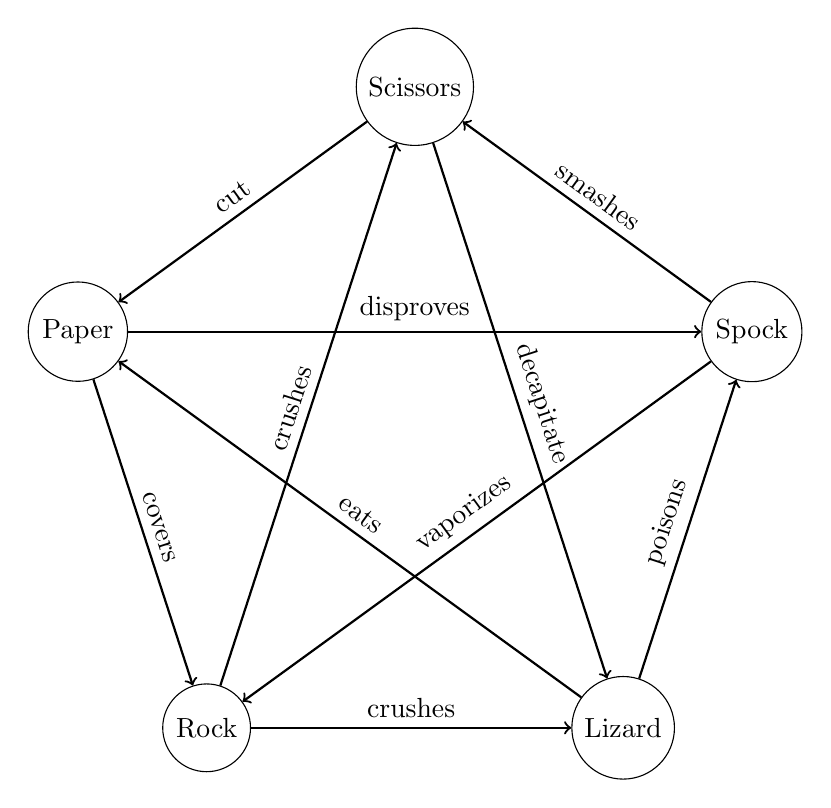
\begin{tikzpicture}

% points
\path (90:4.5cm)    node[shape=circle,draw] (Scissors) {Scissors};
\path (90+1*72:4.5cm) node[shape=circle,draw] (Paper) {Paper};
\path (90+2*72:4.5cm) node[shape=circle,draw] (Rock) {Rock};
\path (90+3*72:4.5cm) node[shape=circle,draw] (Lizard) {Lizard};
\path (90+4*72:4.5cm) node[shape=circle,draw] (Spock) {Spock};

% edges
\tikzstyle{every node}=[above,sloped];

\draw[->,thick] (Scissors) -- node {cut} (Paper);
\draw[->,thick] (Paper) -- node {covers} (Rock);
\draw[->,thick] (Rock) -- node {crushes} (Lizard);
\draw[->,thick] (Lizard) -- node {poisons} (Spock);
\draw[->,thick] (Spock) -- node {smashes} (Scissors);
\draw[->,thick] (Scissors) -- node {decapitate} (Lizard);
\draw[->,thick] (Lizard) -- node {eats} (Paper);
\draw[->,thick] (Paper) -- node {disproves} (Spock);
\draw[->,thick] (Spock) -- node {vaporizes} (Rock);
\draw[->,thick] (Rock) -- node {crushes} (Scissors);

\end{tikzpicture}
\caption{Rock, Paper, Scissors, Lizard, Spock}
\label{fig:rpsls}
\end{figure}



\subsection{Vorgehensweise}
Folgende Punkte sind weiterhin zu beachten:
\begin{itemize}
	\item Es finden regelmäßige Konsultationen mit dem Betreuer oder den Betreuern statt. Grundsätzlich wird ein Serientermin mit zweiwöchentlichem Abstand vereinbart.
	\item Während des Schreibens der Diplom- oder Belegarbeit sollen dem Betreuer regelmäßig im \gls{SVN} des Lehrstuhls Zwischenstände der Ausarbeitung zur Verfügung gestellt werden. Der aktuelle Stand ist dem Betreuer ein bis zwei Tage vor der Konsultation zur Verfügung zu stellen, damit entsprechendes Feedback gegeben werden kann.
	\item Die Verteidigung der Diplom- oder Belegarbeit soll als Beamer-Präsentation durchgeführt werden.
	\item Vor dem Druck sollte die Option \texttt{\textbackslash{}printoutput} aktiviert werden (ganz vorn im Quelltext), damit die bunten Links schwarz werden.
	\item Die Arbeit soll einseitig gedruckt und gebunden sowie als PDF-Dokument abgegeben werden. In der Regel sind zwei gebundene und unterschriebene Exemplare einzureichen. Bei Abschlussarbeiten (Diplomarbeit, Masterarbeit, Bachelorarbeit) muss die Arbeit im Prüfungsamt vor der Einreichung abgestempelt werden.\todo{Eine seitliche Notiz mit \texttt{\textbackslash{}todo\{\}}}
	\item Es müssen die richtigen Fragen \cite{smartquestions} gestellt werden.
	\item Weitere nützliche Hinweise sind unter \cite{seusdiplomfaq} zu finden.
\end{itemize}
\todo[inline]{Eine Inline-Notiz mit \texttt{\textbackslash{}todo[inline]\{\}}}

\subsection{Editoren}
\LaTeX{}-Quelldokumente verwenden als Textdokumente einen Textzeichensatz. Hier kommt mit UTF-8 eine sehr weit verbreitete Umsetzung des global anwendbaren Standards \emph{Unicode} zum Einsatz. Dadurch können Sprachinkompatibilitäten vermieden werden. Diverse \LaTeX{}-Editoren kommen derzeit nicht mit bestimmten bzw. verschiedenen Zeichenkodierungen zurecht.\footnote{Übersicht von verbreiteten Editoren: \url{http://de.wikipedia.org/wiki/LaTeX}} Als guter Editor für viele Plattformen kann \emph{TeXMaker} empfohlen werden.